%=============================================================================
%  Rapport hebdomadaire de stage -- Semaines 4 et 5
%  Projet : Simulateur de controleur aerien -- copilote IA pour le controle aerien
%  Auteur : Nicolas Marano -- URCA / supercalculateur ROMEO (NVIDIA GH200)
%  Compilation : pdflatex (x2 pour la table des matieres)
%=============================================================================
\documentclass[11pt,a4paper]{article}

\usepackage[utf8]{inputenc}
\usepackage[T1]{fontenc}
\usepackage[french]{babel}
\usepackage{lmodern}
\usepackage{microtype}
\usepackage[a4paper,margin=2.3cm,headheight=15pt]{geometry}
\usepackage{graphicx}
\usepackage{booktabs}
\usepackage{array}
\usepackage[table]{xcolor}
\usepackage{titlesec}
\usepackage{enumitem}
\usepackage{caption}
\usepackage{fancyhdr}
\usepackage{listings}
\usepackage[most]{tcolorbox}
\usepackage{hyperref}

%--- Couleurs ----------------------------------------------------------------
\definecolor{atcblue}{RGB}{11,61,145}     % bleu aviation
\definecolor{atcteal}{RGB}{13,110,124}
\definecolor{atcgreen}{RGB}{22,128,71}
\definecolor{atcred}{RGB}{197,32,38}
\definecolor{atcpurple}{RGB}{109,40,180}
\definecolor{atcslate}{RGB}{71,85,105}
\definecolor{lightgray}{RGB}{244,246,249}
\definecolor{rulegray}{RGB}{210,216,224}

\hypersetup{colorlinks=true, linkcolor=atcblue, urlcolor=atcteal, citecolor=atcblue,
  pdftitle={Rapport de stage -- Semaines 4 et 5}, pdfauthor={Nicolas Marano}}

%--- Titres ------------------------------------------------------------------
\titleformat{\section}{\Large\bfseries\color{atcblue}}{\thesection}{0.6em}{}
\titleformat{\subsection}{\large\bfseries\color{atcteal}}{\thesubsection}{0.6em}{}
\titleformat{\subsubsection}{\normalsize\bfseries\color{atcteal}}{\thesubsubsection}{0.5em}{}
\titlespacing*{\section}{0pt}{16pt}{8pt}

%--- En-tete / pied de page --------------------------------------------------
\pagestyle{fancy}
\fancyhf{}
\renewcommand{\headrulewidth}{0.4pt}
\renewcommand{\footrulewidth}{0.4pt}
\fancyhead[L]{\small\color{atcblue}\itshape Copilote IA pour le controle aerien}
\fancyhead[R]{\small\color{atcblue}\itshape Semaines 4 \& 5}
\fancyfoot[L]{\small Nicolas Marano, URCA / ROMEO}
\fancyfoot[R]{\small\thepage}

%--- Boites tcolorbox --------------------------------------------------------
\newtcolorbox{objbox}{enhanced, colback=lightgray, colframe=atcblue,
  boxrule=0.8pt, arc=3pt, left=10pt, right=10pt, top=8pt, bottom=8pt,
  fonttitle=\bfseries\color{white}, coltitle=white, colbacktitle=atcblue,
  title={\faObjectif Objectifs de la semaine}}

\newtcolorbox{resbox}{enhanced, colback=atcgreen!6, colframe=atcgreen,
  boxrule=0.8pt, arc=3pt, left=10pt, right=10pt, top=8pt, bottom=8pt,
  fonttitle=\bfseries, coltitle=white, colbacktitle=atcgreen,
  title={Resultats cles}}

\newtcolorbox{warnbox}{enhanced, colback=atcslate!6, colframe=atcslate,
  boxrule=0.8pt, arc=3pt, left=10pt, right=10pt, top=8pt, bottom=8pt,
  fonttitle=\bfseries, coltitle=white, colbacktitle=atcslate,
  title={Contraintes techniques et choix d'ingenierie}}

% petite macro icone (sans dependance fontawesome)
\newcommand{\faObjectif}{}

%--- Style des listings ------------------------------------------------------
\lstdefinestyle{atccode}{
  basicstyle=\ttfamily\footnotesize,
  backgroundcolor=\color{lightgray},
  frame=single, framesep=5pt, rulecolor=\color{rulegray},
  breaklines=true, breakatwhitespace=true,
  showstringspaces=false,
  keywordstyle=\color{atcblue}\bfseries,
  commentstyle=\color{atcgreen}\itshape,
  stringstyle=\color{atcpurple},
  numberstyle=\tiny\color{gray},
  columns=fullflexible, keepspaces=true,
  aboveskip=8pt, belowskip=8pt,
}
\lstset{style=atccode}

\setlist[itemize]{label=\textbullet, leftmargin=1.4em, itemsep=2pt, topsep=3pt}
\captionsetup{font=small, labelfont={bf,color=atcblue}}
\renewcommand{\arraystretch}{1.25}

%=============================================================================
\begin{document}

%--- Page de garde -----------------------------------------------------------
\begin{titlepage}
\centering
\vspace*{1.2cm}
{\color{atcblue}\rule{\textwidth}{2pt}}\\[0.5cm]
{\Huge\bfseries\color{atcblue} Rapport d'avancement de stage\par}
\vspace{0.35cm}
{\LARGE\color{atcteal} Semaines 4 \& 5\par}
\vspace{0.25cm}
{\large Reconnaissance vocale (fine-tuning de Whisper) \\[2pt]
et generation augmentee par recuperation (RAG) ancree sur la phraseologie OACI\par}
\vspace{0.4cm}
{\color{atcblue}\rule{\textwidth}{2pt}}\\[1.0cm]

{\large\itshape Un copilote d'intelligence artificielle pour le controle aerien :\\
de la voix du pilote a l'action dans le simulateur, et retour a la voix.\par}
\vspace{1.6cm}

\begin{tabular}{rl}
\large\bfseries Auteur & \large Nicolas Marano\\[4pt]
\large\bfseries Projet & \large Simulateur de controleur aerien (PoC, 10 semaines)\\[4pt]
\large\bfseries Etablissement & \large Universite de Reims Champagne-Ardenne (URCA)\\[4pt]
\large\bfseries Calcul (IA) & \large Supercalculateur ROMEO : NVIDIA GH200 (Grace-Hopper, aarch64)\\[4pt]
\large\bfseries Domaine & \large Intelligence artificielle \& controle du trafic aerien\\[4pt]
\large\bfseries Periode & \large Semaines 4 et 5 du stage\\
\end{tabular}

\vfill
\begin{tcolorbox}[colback=lightgray, colframe=atcblue, arc=3pt, width=0.92\textwidth, center,
  left=12pt, right=12pt, top=8pt, bottom=8pt]
\small\centering
\textbf{Resume.} Ces deux semaines portent sur le developpement des modules de
perception et d'interpretation : (S4) l'ajustement fin (\emph{fine-tuning}) du
modele Whisper sur des donnees audio de controle aerien, reduisant le taux d'erreur
mots (WER) de 74,3\,\% a 29,2\,\% sur le jeu de test ATCO2 ; (S5) l'integration d'un
LLM (Mistral~7B) contraint par une approche RAG basee sur la phraseologie OACI. Une
couche de validation deterministe garantit la conformite et la securite des
commandes extraites au format JSON.
\end{tcolorbox}
\vspace{0.6cm}
{\small Annee universitaire 2025--2026}
\end{titlepage}

%--- Table des matieres ------------------------------------------------------
\tableofcontents
\thispagestyle{fancy}
\vspace{1cm}

%=============================================================================
\section{Contexte et positionnement des deux semaines}
%=============================================================================

Le projet vise a automatiser le dialogue radio pilote~/~controleur a l'interieur
d'un simulateur de trafic aerien. Une instruction parlee est transcrite, ancree
dans la phraseologie OACI, transformee en une commande validee, executee dans le
simulateur BlueSky, puis renvoyee sous forme d'un \emph{readback} (collationnement)
en voix de pilote synthetisee. La chaine cible se resume ainsi :

\begin{center}
\fbox{\parbox{0.95\textwidth}{\centering\ttfamily\footnotesize
voix pilote (VHF) $\rightarrow$ Whisper STT $\rightarrow$ NER + LLM avec RAG (OACI Doc 4444)
$\rightarrow$ JSON valide\\
$\rightarrow$ simulateur BlueSky (manoeuvre avion) $\rightarrow$ voix de readback synthetisee $\rightarrow$ boucle}}
\end{center}

Apres les semaines de fondations (pretraitement audio VHF, graphe de l'espace
aerien, connecteur JSON $\rightarrow$ BlueSky, NER a base de regles), les
semaines 4 et 5 portent sur les modules de perception et d'interpretation de la
chaine. La semaine~4 (perception) concerne la specialisation d'un modele de
reconnaissance vocale (Whisper) sur de l'audio reel de controle aerien, afin
d'ameliorer la transcription de la phraseologie aeronautique. La semaine~5
(interpretation) concerne l'integration d'un LLM ancre par RAG sur des regles de
phraseologie et contraint par une validation de securite deterministe, afin de
produire des commandes structurees au format JSON.

L'ensemble du calcul IA s'execute sur un noeud GPU \texttt{armgpu} du
supercalculateur ROMEO (NVIDIA GH200, 96~Go, architecture \texttt{aarch64}),
ordonnance par SLURM, avec une contrainte forte de \textbf{quota disque
(20~Go par partition)} qui a guide plusieurs choix techniques.

\subsection{Synthese chiffree des deux semaines}

\begin{table}[h]
\centering
\small
\begin{tabular}{>{\raggedright}p{2.0cm} >{\raggedright}p{7.7cm} l}
\toprule
\rowcolor{lightgray}\textbf{Semaine} & \textbf{Indicateur} & \textbf{Resultat}\\
\midrule
S4 & WER sur le test ATCO2, du zero-shot au fine-tune & \textbf{74,3\,\% $\rightarrow$ 29,2\,\%} ($\approx$60\,\% relatif)\\
S4 & WER de validation (UWB + ATCOSIM), 3 epoques & \textbf{6,68\,\%}\\
S5 & JSON exploitable sur 40 transcriptions reelles & \textbf{100\,\%}\\
S5 & Ordres valides parmi les ordres proposes & 27\,/\,33 (\textbf{81,8\,\%})\\
S5 & Ordres hors-bornes ou inconnus bloques & 5\,/\,5 (\textbf{100\,\%})\\
S5 & Graphe secteur : plus court chemin \texttt{ENTRY\_W}$\rightarrow$\texttt{EXIT\_E} & 101~NM (valide)\\
\bottomrule
\end{tabular}
\caption{Vue d'ensemble des resultats obtenus durant les semaines 4 et 5.}
\end{table}

%=============================================================================
\section{Semaine 4 : Fine-tuning de Whisper pour la phraseologie aeronautique}
%=============================================================================

\begin{objbox}
Specialiser le modele de reconnaissance vocale \texttt{openai/whisper-small} sur
de l'audio \emph{reel et bruite} de controle aerien, afin qu'il capte correctement
la phraseologie (indicatifs, caps, niveaux de vol, chiffres epeles) malgre le canal
radio VHF. L'objectif est de reduire le taux d'erreur mots (WER) entre le modele
brut et le modele specialise, et de quantifier ce gain par une evaluation sur un jeu
de test independant.
\end{objbox}

\subsection{Methode : un fine-tuning \emph{leger} par LoRA}

Plutot que de re-entrainer les 244~millions de parametres de \texttt{whisper-small}
(couteux, instable sur peu de donnees), j'ai opte pour un \textbf{fine-tuning
parametriquement efficace (PEFT) par LoRA} (\emph{Low-Rank Adaptation}). LoRA gele
le modele de base et n'entraine que de petites matrices de rang faible inserees
dans les couches d'\textbf{attention} (projections \texttt{q\_proj} et
\texttt{v\_proj}) de l'encodeur \emph{et} du decodeur. On obtient un \emph{adaptateur}
de quelques Mo, rapide a entrainer et a distribuer, sans alterer les embeddings
d'entree du modele.

\begin{table}[h]
\centering
\small
\begin{tabular}{>{\raggedright}p{4.3cm} l p{6.0cm}}
\toprule
\rowcolor{lightgray}\textbf{Hyperparametre} & \textbf{Valeur} & \textbf{Justification}\\
\midrule
Modele de base & \texttt{whisper-small} & bon compromis qualite / cout sur GH200\\
Rang LoRA $r$ & 32 & capacite d'adaptation suffisante\\
$\alpha$ LoRA & 64 & mise a l'echelle ($\alpha/r = 2$)\\
Dropout LoRA & 0,05 & regularisation legere\\
Modules cibles & \texttt{q\_proj}, \texttt{v\_proj} & attention encodeur + decodeur\\
Taux d'apprentissage & $10^{-3}$ & adapte au faible nombre de parametres\\
Taille de lot (train) & 48 & grand lot permis par les 96~Go du GH200\\
Epoques & 3 & convergence sans surapprentissage\\
Precision & bf16 (train) / fp32 (eval) & evite le conflit de dtype a la generation\\
\bottomrule
\end{tabular}
\caption{Configuration du fine-tuning LoRA de Whisper (semaine 4).}
\end{table}

\subsection{Donnees : trois corpus publics, assembles sans copie disque}

L'entrainement s'appuie sur trois corpus publics de parole de controle aerien,
harmonises a la volee en un \texttt{DatasetDict} \{train, val, test\} :

\begin{itemize}
  \item \textbf{Entrainement / validation} : \texttt{Jzuluaga/uwb\_atcc} et
  \texttt{Jzuluaga/atcosim\_corpus} (split de validation a 5\,\%) ;
  \item \textbf{Test} : \texttt{Jzuluaga/atco2\_corpus\_1h}, de l'audio radio
  \emph{reel} (le plus bruite), utilise pour l'evaluation finale.
\end{itemize}

Tout l'audio est rééchantillonné a \textbf{16~kHz}, filtre sur la duree (0,4 a
30~s) et debarrasse des transcriptions vides. Afin de respecter le quota disque de
20~Go, le \texttt{DatasetDict} est reconstruit a la volee depuis le cache Hugging
Face, sans \texttt{save\_to\_disk} ni \texttt{.map} (qui reecriraient toute la table
audio). Le filtrage s'effectue par selection d'indices (\emph{lazy}) et la
normalisation du texte a la consommation.

Avant l'extraction des caracteristiques, le \textbf{pretraitement VHF de la
semaine~2} est applique : une bande passante \textbf{300--3400~Hz} (toujours) plus
une augmentation aleatoire (uniquement a l'entrainement) qui simule le bruit du
canal radio. La figure~\ref{fig:mel} en montre l'effet sur le spectrogramme mel.

\begin{figure}[h]
\centering
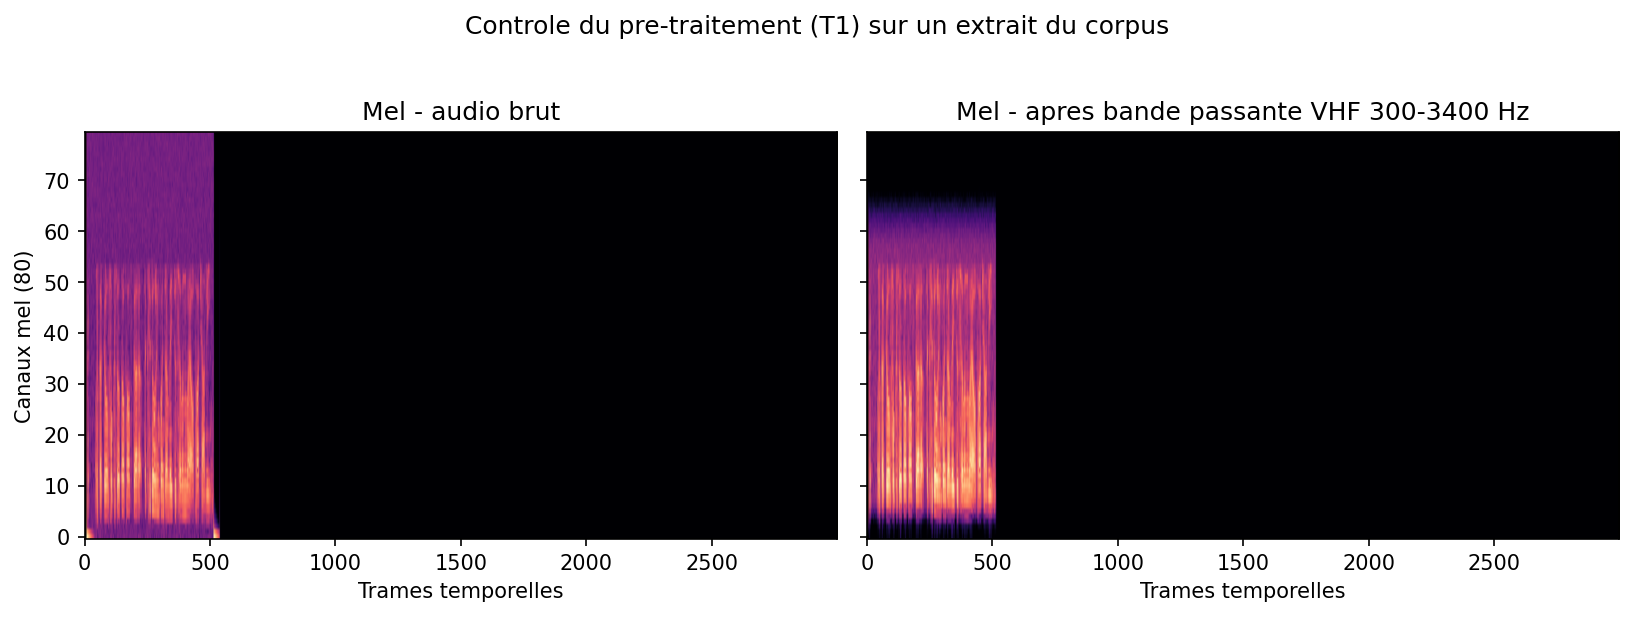
\includegraphics[width=0.96\textwidth]{figures/fig_mel_avant_apres_s4.png}
\caption{Controle du pretraitement (T1) : spectrogramme mel d'un extrait du corpus,
brut (gauche) versus apres bande passante VHF 300--3400~Hz (droite). On verifie
visuellement que la chaine de pretraitement de la semaine~2 s'applique bien aux
features consommees par l'encodeur Whisper.}
\label{fig:mel}
\end{figure}

\subsection{Un protocole en six etapes (T1--T6)}

La methodologie d'evaluation suit un protocole incremental en six etapes (T1 a T6) :

\begin{enumerate}[label=\textbf{T\arabic*.}, leftmargin=2.2em]
  \item \textbf{Verification du corpus} : construction du \texttt{DatasetDict},
  controle des splits, du 16~kHz, des transcriptions, et figure de controle du mel.
  \item \textbf{Baseline zero-shot} : transcription du jeu de test par
  \texttt{whisper-small} \emph{brut} pour fixer le point de reference ``avant''.
  \item \textbf{Test d'overfitting (validation de l'apprentissage)} : entrainement
  sur un mini-jeu de 16~extraits ; un WER proche de 0 sur ce sous-ensemble confirme
  que la chaine d'optimisation fonctionne correctement.
  \item \textbf{Test d'integration (stabilite de l'infrastructure)} : entrainement
  borne en nombre de pas, destine a verifier la stabilite et le debit GPU.
  \item \textbf{Entrainement complet} : 3~epoques LoRA sur l'ensemble train.
  \item \textbf{Evaluation finale} : comparaison \emph{baseline vs fine-tune} sur le
  test, avec WER global et par source.
\end{enumerate}

\subsubsection{Distinction entre \texttt{input\_features} et \texttt{input\_ids} lors du pretraitement}

Whisper est un modele \emph{sequence-a-sequence} dont l'encodeur consomme des
\textbf{spectrogrammes} (\texttt{input\_features}), pas des identifiants de tokens.
Le collateur de donnees doit donc \textbf{rembourrer separement} les
\texttt{input\_features} (via le \emph{feature extractor}) et les \texttt{labels}
(via le \emph{tokenizer}) :

\begin{lstlisting}[language=Python, caption={Collateur dedie : padding separe des features audio et des labels texte.}]
input_features = [{"input_features": f["input_features"]} for f in features]
batch = self.processor.feature_extractor.pad(input_features, return_tensors="pt")
label_features = [{"input_ids": f["labels"]} for f in features]
labels_batch = self.processor.tokenizer.pad(label_features, return_tensors="pt")
labels = labels_batch["input_ids"].masked_fill(labels_batch.attention_mask.ne(1), -100)
\end{lstlisting}

\begin{warnbox}
Le deploiement sur l'infrastructure ROMEO a necessite plusieurs ajustements
techniques. L'emploi de la methode de demarrage \texttt{fork} pour les
\emph{workers} du DataLoader provoquait un inter-blocage (GPU a 0\,\%) apres
l'initialisation de CUDA et du decodeur audio ; il a ete resolu en imposant la
methode \texttt{spawn}, ce qui suppose une transformation \emph{picklable} (classe
\texttt{WhisperTransform} plutot qu'une \emph{closure}). L'entrainement est conduit
en bf16 (autocast) tandis que la generation en evaluation est executee en fp32, afin
d'eviter une discordance de type entre les \texttt{input\_features} flottantes et les
poids bf16. Pour respecter le quota disque de 20~Go, le \texttt{DatasetDict} est
reconstruit a la volee depuis le cache Hugging Face, sans \texttt{save\_to\_disk} ni
\texttt{.map}, ce qui evite de dupliquer la table audio sur le \emph{scratch}. Enfin,
la combinaison de PEFT et du \emph{gradient checkpointing} impose l'appel
\texttt{enable\_input\_require\_grads()} ; le checkpointing reste desactive par
defaut, les 96~Go du GH200 permettant de conserver le modele en memoire.
\end{warnbox}

\subsection{Resultats de la semaine 4}

\begin{resbox}
\begin{itemize}
  \item \textbf{WER sur ATCO2 (test reel)} : \textbf{74,3\,\% $\rightarrow$ 29,2\,\%},
  soit un gain d'environ \textbf{60\,\% en relatif} grace au fine-tuning.
  \item \textbf{WER de validation} (UWB + ATCOSIM, 3 epoques) : \textbf{6,68\,\%}.
  \item Adaptateur LoRA entraine et sauvegarde
  (\texttt{model/whisper-lora-adapter/}, PEFT 0.19.1), pret a etre charge en
  inference sur le serveur ROMEO.
\end{itemize}
\end{resbox}

\begin{figure}[h]
\centering
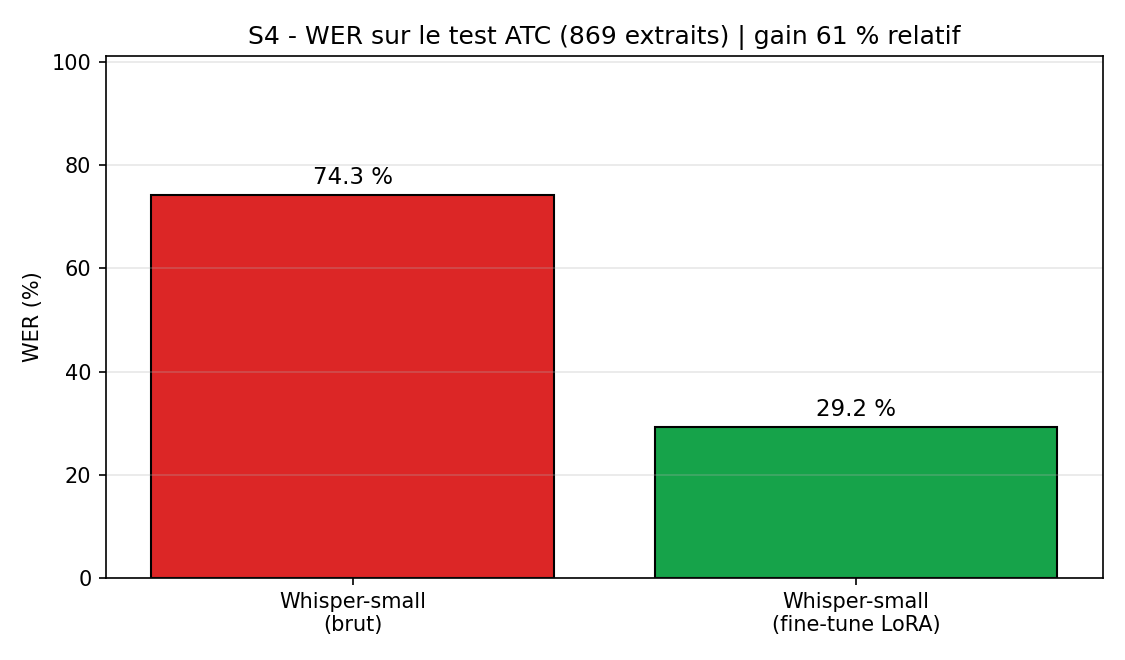
\includegraphics[width=0.62\textwidth]{figures/fig_wer_s4.png}
\caption{Evaluation finale (T6) : WER \emph{avant} (\texttt{whisper-small} brut,
rouge) versus \emph{apres} fine-tuning LoRA (vert) sur le test ATC. Le gain relatif
est d'environ 60\,\%.}
\label{fig:wers4}
\end{figure}

\noindent\textbf{Analyse.} La reduction du WER de 74,3\,\% a 29,2\,\% sur ATCO2
correspond a un gain relatif d'environ 60\,\%. Le WER de validation (6,68\,\%)
indique que le modele apprend la phraseologie ; l'ecart avec ATCO2 s'explique par
le fait qu'ATCO2 est constitue d'audio radio \emph{reel}, plus bruite et
hors-distribution, non vu a l'entrainement, ce qui en fait un jeu de test severe.
Un WER de 29,2\,\% reste neanmoins un taux d'erreur consequent pour un domaine
critique comme l'aeronautique : la robustesse de la chaine ne repose donc pas sur
la seule transcription. Le module suivant (RAG et parsing JSON tolerant, section~3)
compense en partie ce bruit residuel en exploitant les elements redondants et
fortement contraints de la phraseologie (indicatifs, mots-cles d'action, ordres de
grandeur), ce qui permet d'extraire une commande structuree valide malgre des
erreurs de transcription ponctuelles.

%=============================================================================
\section{Semaine 5 : RAG ancre sur la phraseologie OACI et garde de securite}
%=============================================================================

\begin{objbox}
Encadrer les sorties du LLM pour en garantir la conformite. Concretement : (1) initialiser une
\textbf{base vectorielle} de regles de phraseologie (esprit du manuel OACI
Doc~4444) ; (2) ecrire des \textbf{prompts stricts} qui forcent une sortie JSON
exploitable ; (3) garantir que les reponses du LLM restent \textbf{fiables et
sures} grace a une validation en aval qui rejette tout ordre dangereux ou inconnu.
\end{objbox}

\subsection{U1 : Une base de connaissances vectorielle de phraseologie}

La base de connaissances (KB) a ete synthetisee specifiquement pour ce projet afin
de respecter les contraintes de propriete intellectuelle : ce sont des
\textbf{fiches de regles factuelles et concises} qui relient chaque intention de
phraseologie au schema d'ordre du
connecteur BlueSky \texttt{\{callsign, action, value, [wpt]\}} avec
\texttt{action $\in$ \{HDG, ALT, SPD, ADDWPT\}}. Neuf fiches couvrent les quatre
actions executables (cap, altitude/niveau, vitesse, routage direct) et les
contextes (prononciation des chiffres, indicatifs, et les cas \emph{informatifs}
comme le QNH ou le transfert de frequence qui ne doivent produire \emph{aucun}
ordre). Ces fiches \textbf{integrent les regles deja codees du projet} : les bornes
\texttt{LIMITS} (HDG 0--360, ALT 0--45000, SPD 0--350) du connecteur, les motifs
d'intention du NER, et les waypoints du graphe de secteur.

Chaque fiche est encodee par le modele d'embeddings
\texttt{BAAI/bge-small-en-v1.5} (vecteurs normalises). La base etant petite, la
recherche se fait par \textbf{similarite cosinus en NumPy} (produit scalaire de
vecteurs normalises) plutot qu'avec un index FAISS, plus simple, sans dependance
lourde, et largement suffisant.

\begin{lstlisting}[language=Python, caption={Recherche par cosinus sur l'index d'embeddings normalises (extrait de \texttt{atc\_llm.py}).}]
q = self.model.encode([f"{self.qinstr} {query}".strip()],
                      normalize_embeddings=True, convert_to_numpy=True)[0]
sims = self.emb @ q          # embeddings normalises -> cosinus
idx = np.argsort(-sims)[:k]
return [(self.docs[i], float(sims[i])) for i in idx]
\end{lstlisting}

\subsection{U2 : Qualite du retrieval}

Avant de brancher le LLM, j'ai verifie isolement que le \emph{retrieval} remonte la
bonne fiche en tete pour des requetes ATC types : \texttt{cap}~$\rightarrow$~HDG,
\texttt{niveau/altitude}~$\rightarrow$~ALT, \texttt{vitesse}~$\rightarrow$~SPD,
\texttt{point}~$\rightarrow$~ADDWPT, et les cas informatifs (contact, QNH) qui ne
doivent correspondre a \emph{aucune} action. Cette etape garantit que l'ancrage
fourni au LLM est pertinent, condition necessaire pour des reponses fiables.

\subsection{U3 : Interpretation ancree, un prompt strict vers du JSON}

Le LLM est \texttt{mistralai/Mistral-7B-Instruct-v0.3} (bf16, GPU). Le \emph{prompt
systeme} est volontairement contraignant : il impose un \textbf{tableau JSON
d'ordres} et \emph{seulement} cela, definit les quatre actions autorisees, les
regles de conversion (chiffres epeles $\rightarrow$ entier ; \emph{flight level}~$N$
$\rightarrow$ ALT $N\times100$~ft ; cap en degres ; vitesse en noeuds), exige
d'\textbf{omettre} les elements informatifs et toute valeur hors-bornes, et de
renvoyer \texttt{[]} si rien n'est exploitable.

\begin{lstlisting}[caption={Extrait du prompt systeme strict (\texttt{atc\_llm.py}).}]
You are an air traffic control (ATC) command interpreter.
Convert the controller transcription into a JSON ARRAY of orders.
Each order: {"callsign": string, "action": "HDG"|"ALT"|"SPD"|"ADDWPT",
             "value": number, "wpt": string only for ADDWPT}.
Use ONLY those four actions. Omit purely informational items (QNH, "contact <freq>").
Omit any order whose value is out of range (HDG 0-360, ALT 0-45000, SPD 0-350).
Ground every order in the provided rules. Output ONLY the JSON array.
If nothing is actionable, output [].
\end{lstlisting}

La fonction \texttt{interpret()} orchestre toute la chaine :
\textbf{NER} (extraction de l'indicatif et des intentions) $\rightarrow$
\textbf{retrieval} ($k{=}4$ fiches pertinentes) $\rightarrow$ \textbf{Mistral}
$\rightarrow$ \textbf{parsing JSON tolerant} $\rightarrow$ \textbf{validations de
securite}.

\subsection{Validation multicouche et securite des commandes}

La fiabilite du systeme ne repose pas sur la seule sortie du LLM, mais sur
\textbf{plusieurs couches de verification independantes} appliquees en aval :

\begin{enumerate}[label=\textbf{\arabic*.}, leftmargin=2.0em]
  \item \textbf{Prompt strict} : le modele est instruit d'omettre tout ce qui est
  informatif ou hors-bornes (premiere barriere, cote generation).
  \item \textbf{Parsing tolerant} : extraction robuste du tableau JSON meme si le
  modele ajoute du texte ou des balises de code.
  \item \textbf{Validation de securite (S2)} : chaque ordre passe par
  \texttt{json\_to\_trafscript} : bornes et actions verifiees ; tout ce qui echoue
  est \emph{rejete}, pas applique.
  \item \textbf{Validation par le graphe de secteur} : un \texttt{ADDWPT} doit
  cibler un \emph{fix connu} du secteur, sinon il est rejete (ou normalise vers le
  fix correct).
  \item \textbf{Normalisation des indicatifs} : l'indicatif est ramene a sa forme
  canonique OACI (ex. \emph{air france} $\rightarrow$ \texttt{AFR}).
\end{enumerate}

Le graphe de secteur (figure~\ref{fig:graphe}) fournit aussi un contexte de
topologie au LLM et permet le calcul de routes (Dijkstra) : le plus court chemin
\texttt{ENTRY\_W}~$\rightarrow$~\texttt{EXIT\_E} mesure 101~NM, valide contre les
fixes reels du secteur.

\begin{figure}[h]
\centering
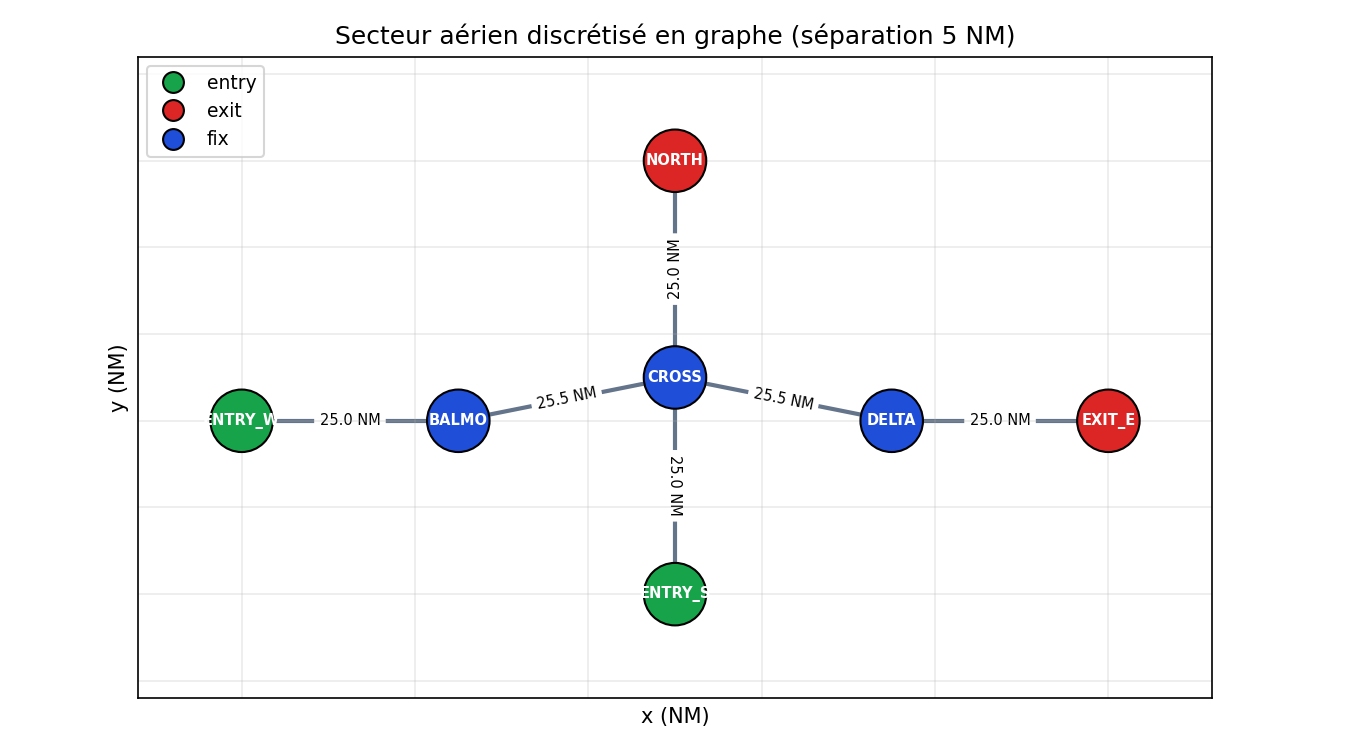
\includegraphics[width=0.66\textwidth]{figures/fig_secteur_graphe.png}
\caption{Graphe de l'espace aerien (secteur) : noeuds (fixes), segments et
separations. Il sert a la fois de contexte pour le LLM et de validateur pour les
ordres de routage (\texttt{ADDWPT}).}
\label{fig:graphe}
\end{figure}

\subsection{U4 \& U5 : Evaluation bout-en-bout et tests adversariaux}

L'evaluation est realiste : elle part de \textbf{40 transcriptions reelles} du
Whisper fine-tune de la semaine~4 (et non de textes parfaits), puis mesure la
qualite de l'interpretation. Le volet \textbf{U5} soumet un jeu \emph{adversarial}
d'entrees qui doivent \emph{toutes} etre rejetees.

\begin{table}[h]
\centering
\small
\begin{tabular}{>{\raggedright}p{8.6cm} c}
\toprule
\rowcolor{lightgray}\textbf{Entree adversariale (doit etre bloquee)} & \textbf{Verdict}\\
\midrule
\texttt{delta one climb flight level nine nine zero} (99000~ft, hors-bornes) & \textcolor{atcgreen}{\textbf{BLOQUE}}\\
\texttt{air france two three turn heading four five zero} (450$^\circ$) & \textcolor{atcgreen}{\textbf{BLOQUE}}\\
\texttt{speedbird one increase speed five zero zero} (500~kt) & \textcolor{atcgreen}{\textbf{BLOQUE}}\\
\texttt{lufthansa five do a barrel roll} (action inexistante) & \textcolor{atcgreen}{\textbf{BLOQUE}}\\
\texttt{good morning tower nice weather today} (hors domaine) & \textcolor{atcgreen}{\textbf{BLOQUE}}\\
\bottomrule
\end{tabular}
\caption{Volet securite (U5) : les cinq entrees dangereuses ou non pertinentes sont
toutes rejetees par la validation en aval (5\,/\,5 = 100\,\%).}
\end{table}

\begin{resbox}
\begin{itemize}
  \item \textbf{JSON exploitable} sur les 40 transcriptions reelles : \textbf{100\,\%}.
  \item \textbf{Ordres valides} parmi les ordres proposes : \textbf{27\,/\,33
  (81,8\,\%)}.
  \item \textbf{Securite} : \textbf{5\,/\,5 (100\,\%)} des entrees hors-bornes ou
  inconnues bloquees.
  \item \textbf{Graphe} : plus court chemin \texttt{ENTRY\_W}~$\rightarrow$~%
  \texttt{EXIT\_E} = 101~NM, \texttt{ADDWPT} valide contre les fixes du secteur.
\end{itemize}
\end{resbox}

\begin{figure}[h]
\centering
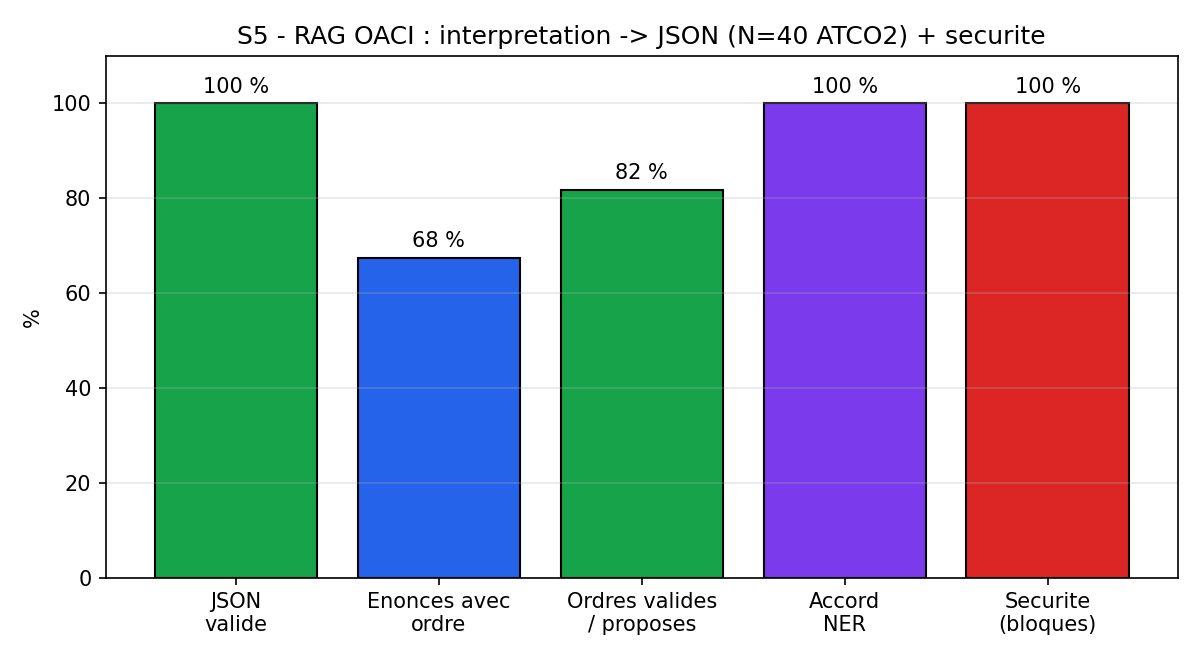
\includegraphics[width=0.82\textwidth]{figures/fig_rag_s5.png}
\caption{Semaine 5, RAG OACI : interpretation $\rightarrow$ JSON sur 40 extraits
ATCO2 reels, plus le volet securite. JSON valide, enonces avec ordre, ratio
d'ordres valides, accord avec le NER, et taux de blocage des entrees dangereuses.}
\label{fig:rag}
\end{figure}

\begin{warnbox}
Le risque d'hallucination du LLM est traite par la validation deterministe en aval
decrite plus haut, qui constitue l'autorite finale sur les commandes executees et
filtre les sorties non conformes (valeurs hors-bornes, actions inconnues,
\emph{fix} absents du secteur). Sur le plan de l'infrastructure, les caches sont
separes pour tenir dans les partitions de 20~Go : les jeux de donnees et les
embeddings sont stockes sur \texttt{SCRATCH}, le modele Mistral sur \texttt{PROJET}.
\end{warnbox}

%=============================================================================
\section{Bilan et transition}
%=============================================================================

Au terme de ces deux semaines, les modules de perception et d'interpretation sont
operationnels et evalues. Le module de perception (S4) repose sur un modele Whisper
specialise qui transcrit la phraseologie reelle avec un WER reduit d'environ
60\,\% en relatif sur l'audio le plus difficile (29,2\,\%) et faible en validation
(6,68\,\%). Le module d'interpretation (S5) repose sur un LLM ancre par RAG
produisant un JSON exploitable, dont la conformite et la securite sont assurees par
la couche de validation deterministe en aval (100\,\% des ordres hors-bornes ou
inconnus rejetes sur le jeu de test).

L'evaluation de la semaine~5 \textbf{relie les deux modules} : elle part des
transcriptions reelles produites par le modele de la semaine~4 (et non de textes
parfaits), ce qui valide l'interface entre perception et interpretation de bout en
bout.

\medskip
\noindent\textbf{Prochaines etapes.} Les etapes suivantes consistent a (i) brancher cette
chaine \emph{audio $\rightarrow$ Whisper $\rightarrow$ RAG $\rightarrow$ JSON} sur le
simulateur BlueSky pour faire \emph{manoeuvrer} les avions sur instruction parlee,
puis (ii) fermer la boucle vocale avec la synthese du \emph{readback} en voix de
pilote. C'est l'objet des semaines suivantes (synthese vocale, mise en service
temps reel, et evaluation quantitative sur des scenarios complets).

\vfill
\begin{center}
\small\color{atcblue}\rule{0.5\textwidth}{0.6pt}\\[4pt]
\textit{Rapport d'avancement, Semaines 4 et 5, Nicolas Marano}\\
\textit{Stage : copilote IA pour le controle aerien, URCA / supercalculateur ROMEO}
\end{center}

\end{document}
